\documentclass{article}
\usepackage[utf8]{inputenc}
\usepackage{fancyhdr}
\usepackage{lastpage}
\usepackage{amsfonts}
\usepackage{graphicx}
\usepackage{amsmath}
\usepackage{amssymb}
\usepackage{bm}

\usepackage[shortlabels]{enumitem}
\usepackage[noabbrev, capitalise]{cleveref}

\usepackage{geometry}
 \geometry{
 a4paper,
 top=20mm,
 bottom=25mm,
 left=25mm,
 right=25mm,
 }

\newcommand{\firststudentid}{315140830}
\newcommand{\secondstudentid}{322532102}
\newcommand{\thirdstudentid}{213144173}

\pagestyle{fancy}
\fancyhf{}
\rhead{Solution for Assignment 2}
\chead{\firststudentid \qquad \secondstudentid \qquad \thirdstudentid}
\lhead{Natural Language Processing}
\rfoot{Page \thepage \hspace{1pt} of \pageref{LastPage}}
\renewcommand{\footrulewidth}{1pt}
 
\setlength{\parindent}{0pt}
\setlength{\parskip}{1em}
\renewcommand{\baselinestretch}{1.25}

\renewcommand{\thesubsection}{\thesection.\alph{subsection}}
\renewcommand{\thesubsubsection}{\thesubsection.\roman{subsubsection}}

\begin{document}

\section{Word-Level Neural Bi-gram Language Model}
\subsection{}
\noindent
Starting from our fundamental cross-entropy definition:
\[ \text{CE}(y, \hat{y}) = -\sum_i y_i \cdot \log(\hat{y}_i) \]

\noindent
For a word-level model with softmax output, we can express $\hat{y}_i$ as:
\[ \hat{y}_i = \text{softmax}(\theta)_i = \frac{\exp(\theta_i)}{\sum_j \exp(\theta_j)} \]

\noindent
Let's derive the gradient. For any output $k$ (where $y$ is the one-hot vector):

\begin{align}
\frac{\partial \text{CE}}{\partial \theta_k} &= 
-\sum_i y_i \cdot \frac{\partial}{\partial \theta_k} \log(\hat{y}_i) \\[1em]
&= -\sum_i y_i \cdot \frac{\partial}{\partial \theta_k} \log\left(\frac{\exp(\theta_i)}{\sum_j \exp(\theta_j)}\right) \\[1em]
&= -\sum_i y_i \cdot \left(\delta_{ik} - \hat{y}_k\right) \\[1em]
&= \hat{y}_k - y_k
\end{align}

\noindent
Therefore, we can concisely express the gradient as:
\[ \frac{\partial \text{CE}}{\partial \theta} = \hat{y} - y \]

\noindent
where $y$ is the one-hot target vector and $\hat{y}$ is the predicted probability distribution.
\subsection{}

\noindent
Following the chain rule of differentiation, we can express the gradient as:

\begin{align*}
\frac{\partial J}{\partial x} &= \frac{\partial J}{\partial(hW_2 + b_2)} \cdot \frac{\partial(hW_2 + b_2)}{\partial h} \cdot \frac{\partial \sigma}{\partial(xW_1 + b_1)} \cdot \frac{\partial(xW_1 + b_1)}{\partial x} \\[1em]
&= (\hat{y} - y) \cdot W_2^\top \odot (h(1-h)) \cdot W_1^\top
\end{align*}

\noindent
This derivation shows the complete backward propagation of the gradient through the neural network layers, accounting for the weights ($W_1$, $W_2$), biases ($b_1$, $b_2$), and the activation function's derivative.
\subsection{}
Code is attached.
\subsection{}
After training the network for 40K iterations, we got 113.699 dev perplexity.

\section{Generating Shakespeare Using a Character-level Language Model}
\subsection{}
\textbf{Advantages of Character-Based Language Models:} 

Character-based models can handle any word, even unseen words or words that are not in the vocabulary. They have a smaller vocabulary compared to word-based models, which makes them more efficient in terms of memory. Additionally, they can capture subtleties like prefixes, suffixes, or spelling variations better than word-based models.

\textbf{Advantages of Word-Based Language Models:} 

Word-based models are faster to train because they process fewer tokens for the same text length. They are also able to achieve better syntactic and semantic understanding, resulting in more coherent and meaningful text generation.
\subsection{Graph Plot}
\begin{figure}[h!]
    \centering
    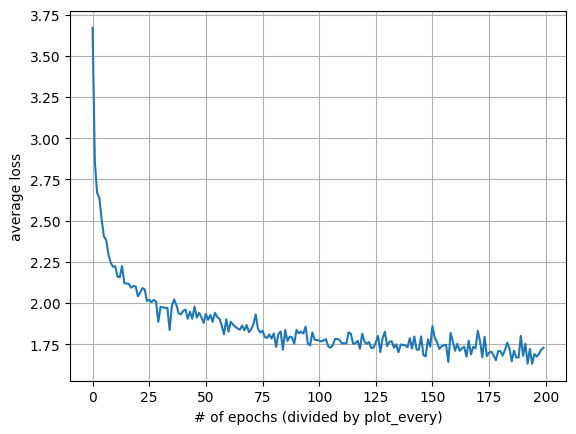
\includegraphics[width=0.5\textwidth]{loss:epochs shakesepeer model}
    \caption{Average loss over epochs}
    \label{fig:example}
\end{figure}

\section{Perplexity}
\subsection{}
\begin{align*}
2^{-\frac{1}{M} \sum_{i=1}^{M} \log_2 P(s_i \mid s_1, \dots, s_{i-1})} 
&= \left(2^{\sum_{i=1}^{M} \log_2 P(s_i \mid s_1, \dots, s_{i-1})}\right)^{-\frac{1}{M}} \\
&= \left(2^{\log_2 P(s_1) + \log_2 P(s_2 \mid s_1) + \dots + \log_2 P(s_M \mid s_1, \dots, s_{M-1})}\right)^{-\frac{1}{M}} \\
&= \left(P(s_1) \cdot P(s_2 \mid s_1) \cdot \dots \cdot P(s_M \mid s_1, \dots, s_{M-1})\right)^{-\frac{1}{M}} \\
&= \left(e^{\ln P(s_1) + \ln P(s_2 \mid s_1) + \dots + \ln P(s_M \mid s_1, \dots, s_{M-1})}\right)^{-\frac{1}{M}} \\
&= \left(e^{\sum_{i=1}^{M} \ln P(s_i \mid s_1, \dots, s_{i-1})}\right)^{-\frac{1}{M}} \\
&= e^{-\frac{1}{M} \sum_{i=1}^{M} \ln P(s_i \mid s_1, \dots, s_{i-1})}.
\end{align*}
\subsection{}
\textbf{Neural Bi-gram Language Model:}

Shakespeare Perplexity:
7.122318650322853

Wikipedia Perplexity:25.75261330172207

\textbf{Character-level Language
Model:}

Shakespeare Perplexity: 7.459401319332429

Wikipedia Perplexity: 19.97325117242642
\subsection{}
For the Character-level Language Model we can assume those result are due to the fact that he learns at the charachter level and also was trained on shakespear data which can give the advantage to more similiar text who is also contains non standard spelling and word forms but on the other hand the result on wikipedia was worse to the more complex and structured word level patterns.
For the Bi-gram Model we would assume it struggled with Wikipedia and got even a worse score than the character-level language model because it is limited to a 2 word context, where in Wikipedia text usually contains long sentences with dependencies that span multiple words. Our assumption that the score is even lower then the Character-level Language Model to the the later ability to capture meanings of suffixes, prefixes even in complex modern words while not relying on find word pairs.
Also we think the the Bi-gram model performs better on shakespear because the word pairs and sentence structures in shakespeares text are relatively predictable and consistent .
\subsection{}
\textbf{Neural Bi-gram Language Model: (After preprocessing)}

Shakespeare Perplexity: 4.475288916573775

Wikipedia Perplexity: 2.536595085380771

\textbf{Character-level Language
Model: (After preprocessing)}

Shakespeare Perplexity: 6.740292861033496

Wikipedia Perplexity: 16.24853261546454

During preprocessing, we primarily focused on "cleaning" the data. This included converting all text to lowercase for better generalization, removing all non-printable characters (which are likely irrelevant to the context), and eliminating extra spaces.

\section{Deep Averaging Networks}
\subsection{}
YOUR ANSWER HERE
\subsection{}
YOUR ANSWER HERE
\subsection{}
YOUR ANSWER HERE
\subsection{}
YOUR ANSWER HERE
\subsection{}
YOUR ANSWER HERE

\section{Attention Exploration}
\subsection{1.a}
\subsubsection{}
\(\alpha\) can be interpreted as categorial probability distribution because:

1. \(\alpha_i > 0\) for each \(i \in [n]\) due to the \(\exp(x)\) function properties.

2. \[
\sum_{i=1}^n \alpha_i = \sum_{i=1}^n \frac{\exp(k_i^\top q)}{\sum_{j=1}^n \exp(k_j^\top q)} = 
\frac{\sum_{i=1}^n \exp(k_i^\top q)}{\sum_{j=1}^n \exp(k_j^\top q)} = 1.
\]

since \(\alpha\) hold those two conditions it can be interpreted as categorial probability distribution.

\subsubsection{}
\(\alpha_j\) is dependent on \(k_j\) and \(q\), so in order to achieve \(\alpha_j \gg \sum_{i \neq j} \alpha_i\), we would want \(k_j \gg k_i\) for each \(i \neq j\) in \([n]\).
\subsubsection{}
Since \(\alpha_j \gg \sum_{i \neq j} \alpha_i\), we can presume \(\alpha_j \approx 1\). 

And since \(c = \sum_{i=1}^n v_i \alpha_i \approx 1 \cdot v_j = v_j\), it means we will get \(c\) that is very close to \(v_j\).
\subsubsection{}
It means that if the product between one of the key vectors and the query is very large compared to the other keys, then that query and the key are similar. This is because the output of the attention will be very close to the value associated with that key.
\subsection{}
\subsubsection{}
First, let's take a look at \( \text{Ms} \):
\[
\text{Ms} = M(v_a + v_b) = Mv_a + Mv_b = M(c_1a_1 + c_2a_2 + \dots + c_n a_n) + M(d_1b_1 + d_2b_2 + \dots + d_m b_m)
\]
\[
= MAc + MBd
\]
where 
\[
c = \begin{pmatrix} c_1 \\ \vdots \\ c_n \end{pmatrix}, \quad d = \begin{pmatrix} d_1 \\ \vdots \\ d_m \end{pmatrix}
\]

Since \( Ac = v_a \) and \( Bd = v_b \), we can use the orthogonal properties of both bases and choose \( M = AA^T \), yielding:
\[
MAc = MBd = A A^T c + A A^T B d = A I c + A^* 0 d = A c = v_a
\]

\subsubsection{}
First, since \( c \approx \frac{1}{2} (v_a + v_b) \), we get \( \alpha_a = \alpha_b = \frac{1}{2} \). From equation (1a), we can deduce that this implies \( k_a^T q + k_b^T q \gg k_i^T q \), for each \( i \neq a, b \in [n] \).

Now, if we choose \( q = \beta (k_a + k_b) \), with \( \beta \gg 0 \), we will get:
\[
\alpha_i = \left\{
\begin{array}{ll}
\frac{\exp(\beta)}{n - 2 + 2 \exp(b)} & \text{if } i = a \text{ or } i = b, \\
\frac{\exp(0)}{n - 2 + 2 \exp(\beta)} & \text{if } i \neq a, b.
\end{array}
\right.
\]
Since \( \beta \gg 0 \), we have \( \exp(\beta) \to \infty \), which means:
\[
\alpha_i = \left\{
\begin{array}{ll}
\frac{1}{2} & \text{if } i = a \text{ or } i = b, \\
0 & \text{if } i \neq a, b.
\end{array}
\right.
\]
as wanted.

\subsection{}
YOUR ANSWER HERE
\subsection{}
YOUR ANSWER HERE


\end{document}
